Aus \autoref{fig:Aufbau} lässt sich der ungefähre Aufbau entnehmen, über das Digitalvoltmeter lässt sich die Temperatur bestimmen, als Referenz für das Digitalvoltmeter wird ein Thermoelement in $\SI{0}{\celsius}$ kaltes Wasser gelegt, wobei darauf geachtet werden sollte, dass das kalte Wasser am Boden $\SI{4}{\celsius}$ hat.
Im Experiment soll $C_p$ bestimmt werden.\\

\begin{wrapfigure}[16]{r}{0.4\textwidth}
	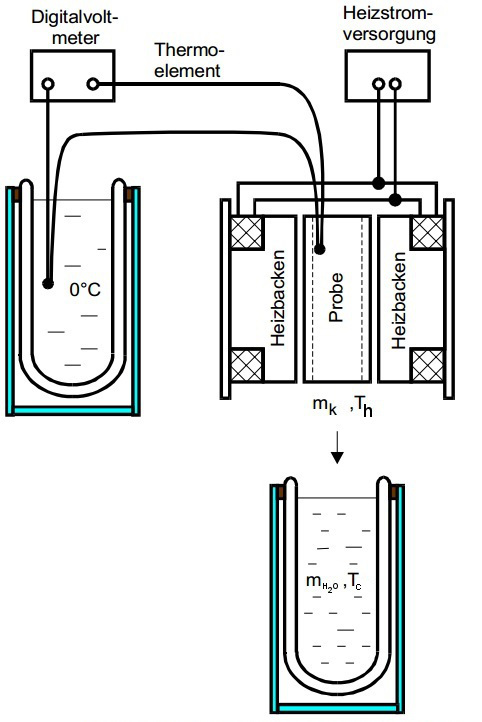
\includegraphics[scale=0.5]{Grafiken/Aufbau.jpg}
	\caption{Schematische Darstellung der Messapparatur (leicht verändert aus \cite{V201})}
	\label{fig:Aufbau}
\end{wrapfigure}
Als erstes werden dafür die Probenkörper in einem Wasserbad erhitzt bis
das Wasser zu kochen anfängt, währenddessen wird noch die Temperatur $T_c$ des Wassers im kalten Messbecher ermittelt. Die Temperatur $T_h$ des kochenden Wassers wird gemessen um einen Vergleichswert für den Fehler des Aufbaus zu bekommen.
Der erhitzte Probenkörper (in unserem Fall Kupfer und Aluminium) wird nun in das kalte Wasser gesetzt und nach einer Minute die Temperatur des Mischwassers ermittelt.
Zum Schluss wird noch die spezifische Wärmekapazität des Wassers ermittelt, da uns natürlich nur $C_p$ von Kupfer bzw. Aluminium interessiert. Dies geschieht auf die selbe Art und Weise, allerdings wird 
vorher noch bestimmt wie viel erhitztes Wasser in das kalte Wasser gegeben werden muss, da die Masse gleich bleiben soll.
